% !TEX root = ../main.tex
%
\chapter{Application Design}
\label{sec:design}

\section{Design Process}
\label{sec:design:ux}

The transition from initial user research findings to a functional prototype was a multi-step process focused on capturing user needs and translating them into a tangible design. 
This section outlines the journey from abstract requirements to the creation of the prototype, emphasizing the methodologies employed at each step.

\subsection*{From User Research to User Flow Diagram}

Following the completion of initial user research, the first step involved modeling the key findings into a user flow diagram (Figure \ref{fig:design:flow-1}).
This diagram served as a visual representation of the user's journey through the prototype, highlighting the main actions, decisions, and interactions users would have with the system. 

\begin{figure}[htb]
	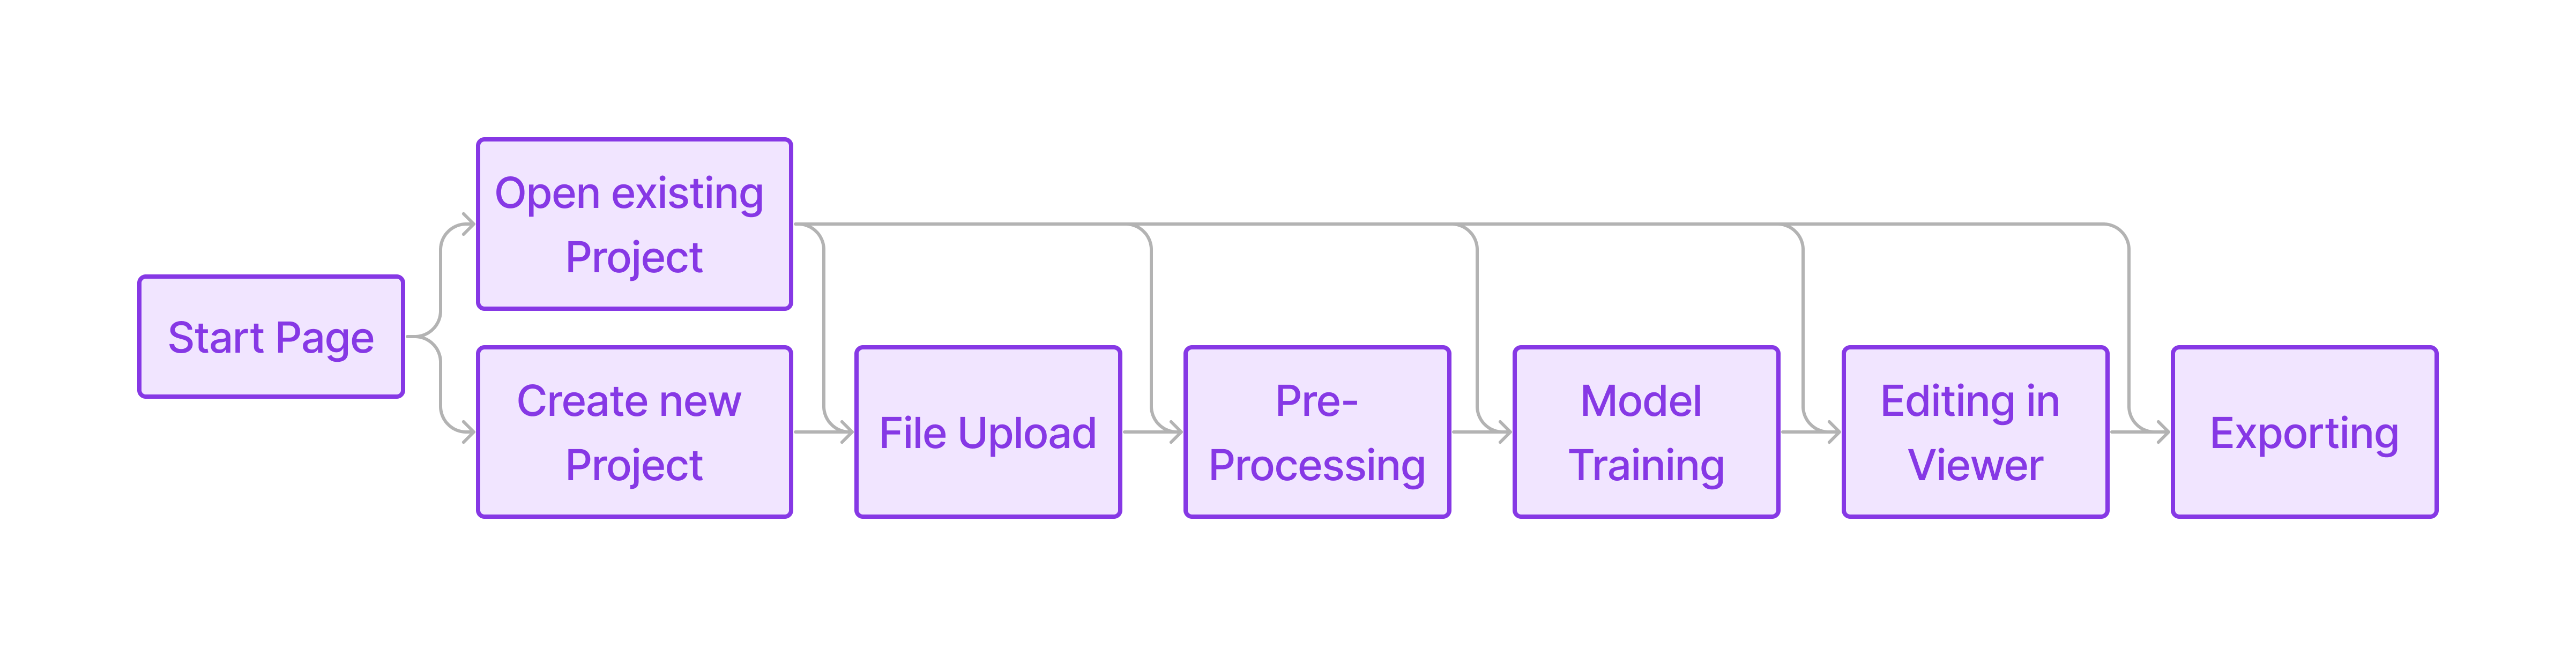
\includegraphics[width=\textwidth]{figures/flow-1.png}
	\caption{User Flow Diagram}
	\label{fig:design:flow-1}
\end{figure}

The purpose of the user flow diagram was not only to map out the envisioned user experience but also to identify any potential bottlenecks or usability issues early in the design process.

\subsection*{Developing the Site Map}

Building on the foundation laid by the user flow diagram, the next step was to expand this outline into a detailed site map. 
The site map provided a more comprehensive view of the prototype's structure, detailing the relationships between different pages and features. 
This excerpt from the site map (Figure \ref{fig:design:flow-2}) illustrates the level of detail and complexity involved in mapping out the prototype's user interactions.

\begin{figure}[htb]
  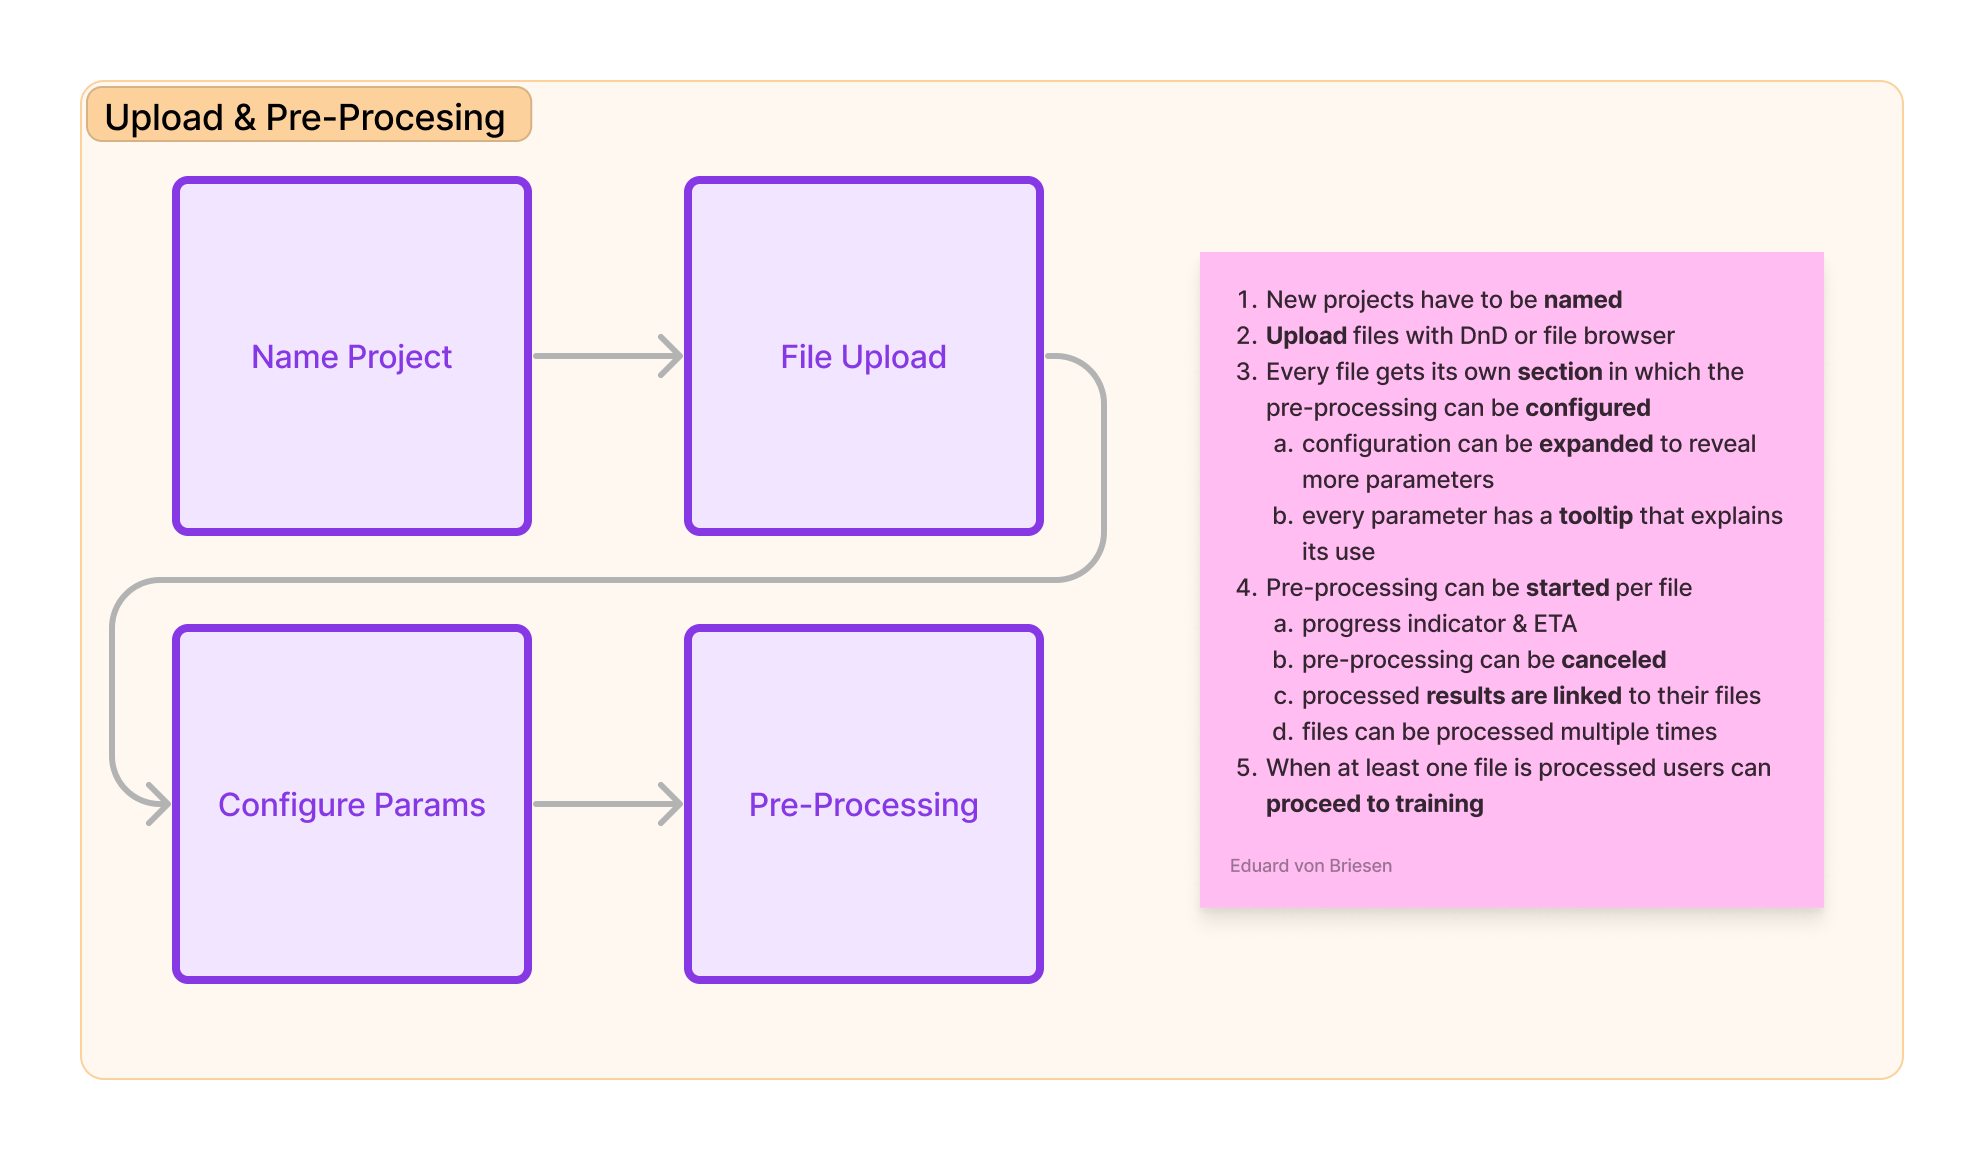
\includegraphics[width=\textwidth]{figures/flow-2.png}
  \caption{Excerpt of a View from the Flow Diagram with detailed interactions}
  \label{fig:design:flow-2}
\end{figure}

This expanded view was instrumental in ensuring that the user flow remained intuitive across the broader system, facilitating easy navigation and a cohesive user experience.

\subsection*{Wireframing}

With a solid understanding of the user flow and site structure, the focus shifted to wireframing. 
Initial wireframes were created to model the overall layout of the interface, providing a skeletal framework for the visual design. 
These wireframes were kept intentionally simple to prioritize structural and functional decisions over aesthetic considerations.
At this stage, emphasis was placed on the placement of key elements, usability, and adherence to the user flow and site map.

\begin{figure}[htb]
  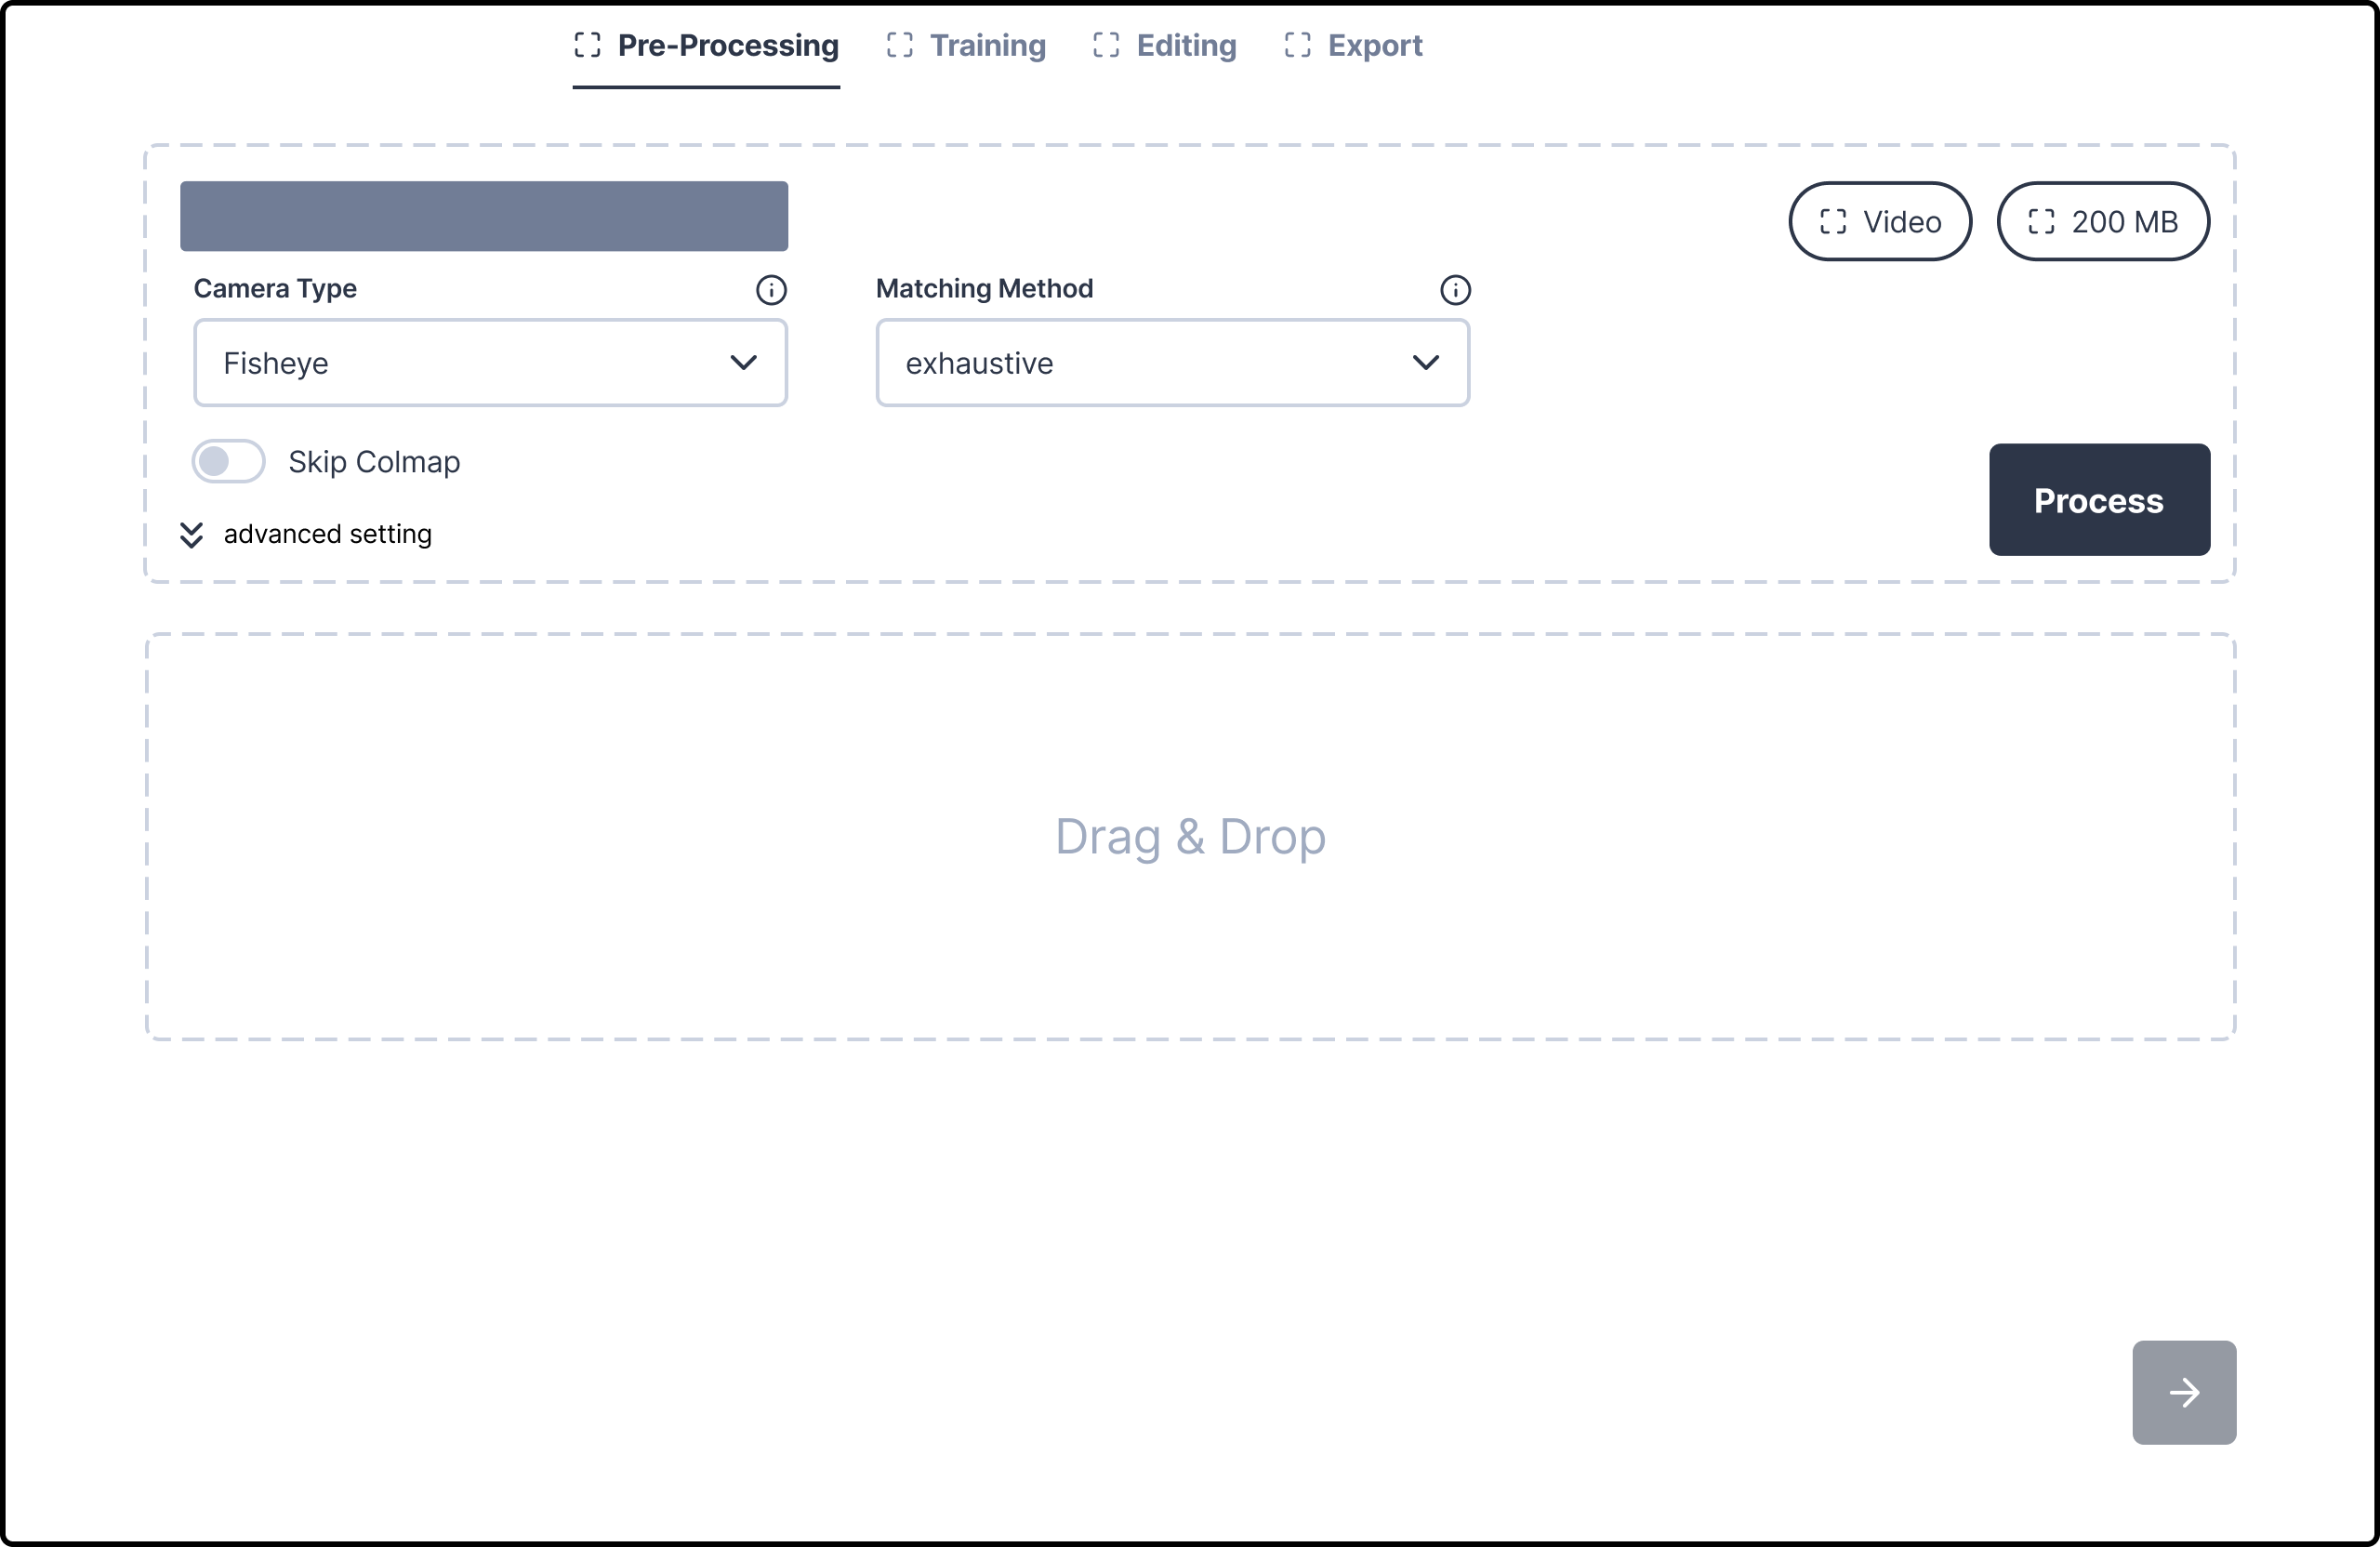
\includegraphics[width=\textwidth]{figures/wireframe.png}
  \caption{Wireframe of the Pre-Processing Section}
  \label{fig:design:wireframe}
\end{figure}

\subsection*{Refinement Through Development}

The transition from wireframes to a working prototype involved iterative refinement during the development phase. 
As the prototype took shape, initial designs were continuously evaluated and adjusted based on practical considerations and technical constraints. 
This phase allowed for a deeper exploration of interactions, animations, and the overall look and feel of the interface. 
It was during this time that the wireframes evolved into a more detailed and user-friendly interface, with adjustments made as necessary to enhance usability and ensure a seamless user experience.

\section{User Interface Design}
The user interface was designed to be as simple as possible, while still providing all necessary functionality. 
The design of the prototype can be broken down into two main parts: a dashboard that gives an overview of all projects and a project section that provides users with the tools to create and edit NeRF models.

\subsection*{Dashboard}

The dashboard is the first view that users see when opening the application. It shows all previously created projects and allows users to create new ones. 
Projects are represented as cards, showing the project name, a preview of on the provided input images (if present), and tags the indicate the current status of the project.
An additional card is present through which users can create a new project, by providing a name.
Projects can be opened by clicking a button on the respective card, when creating a new project, users are redirected to the project section.

\begin{figure}[htb]
  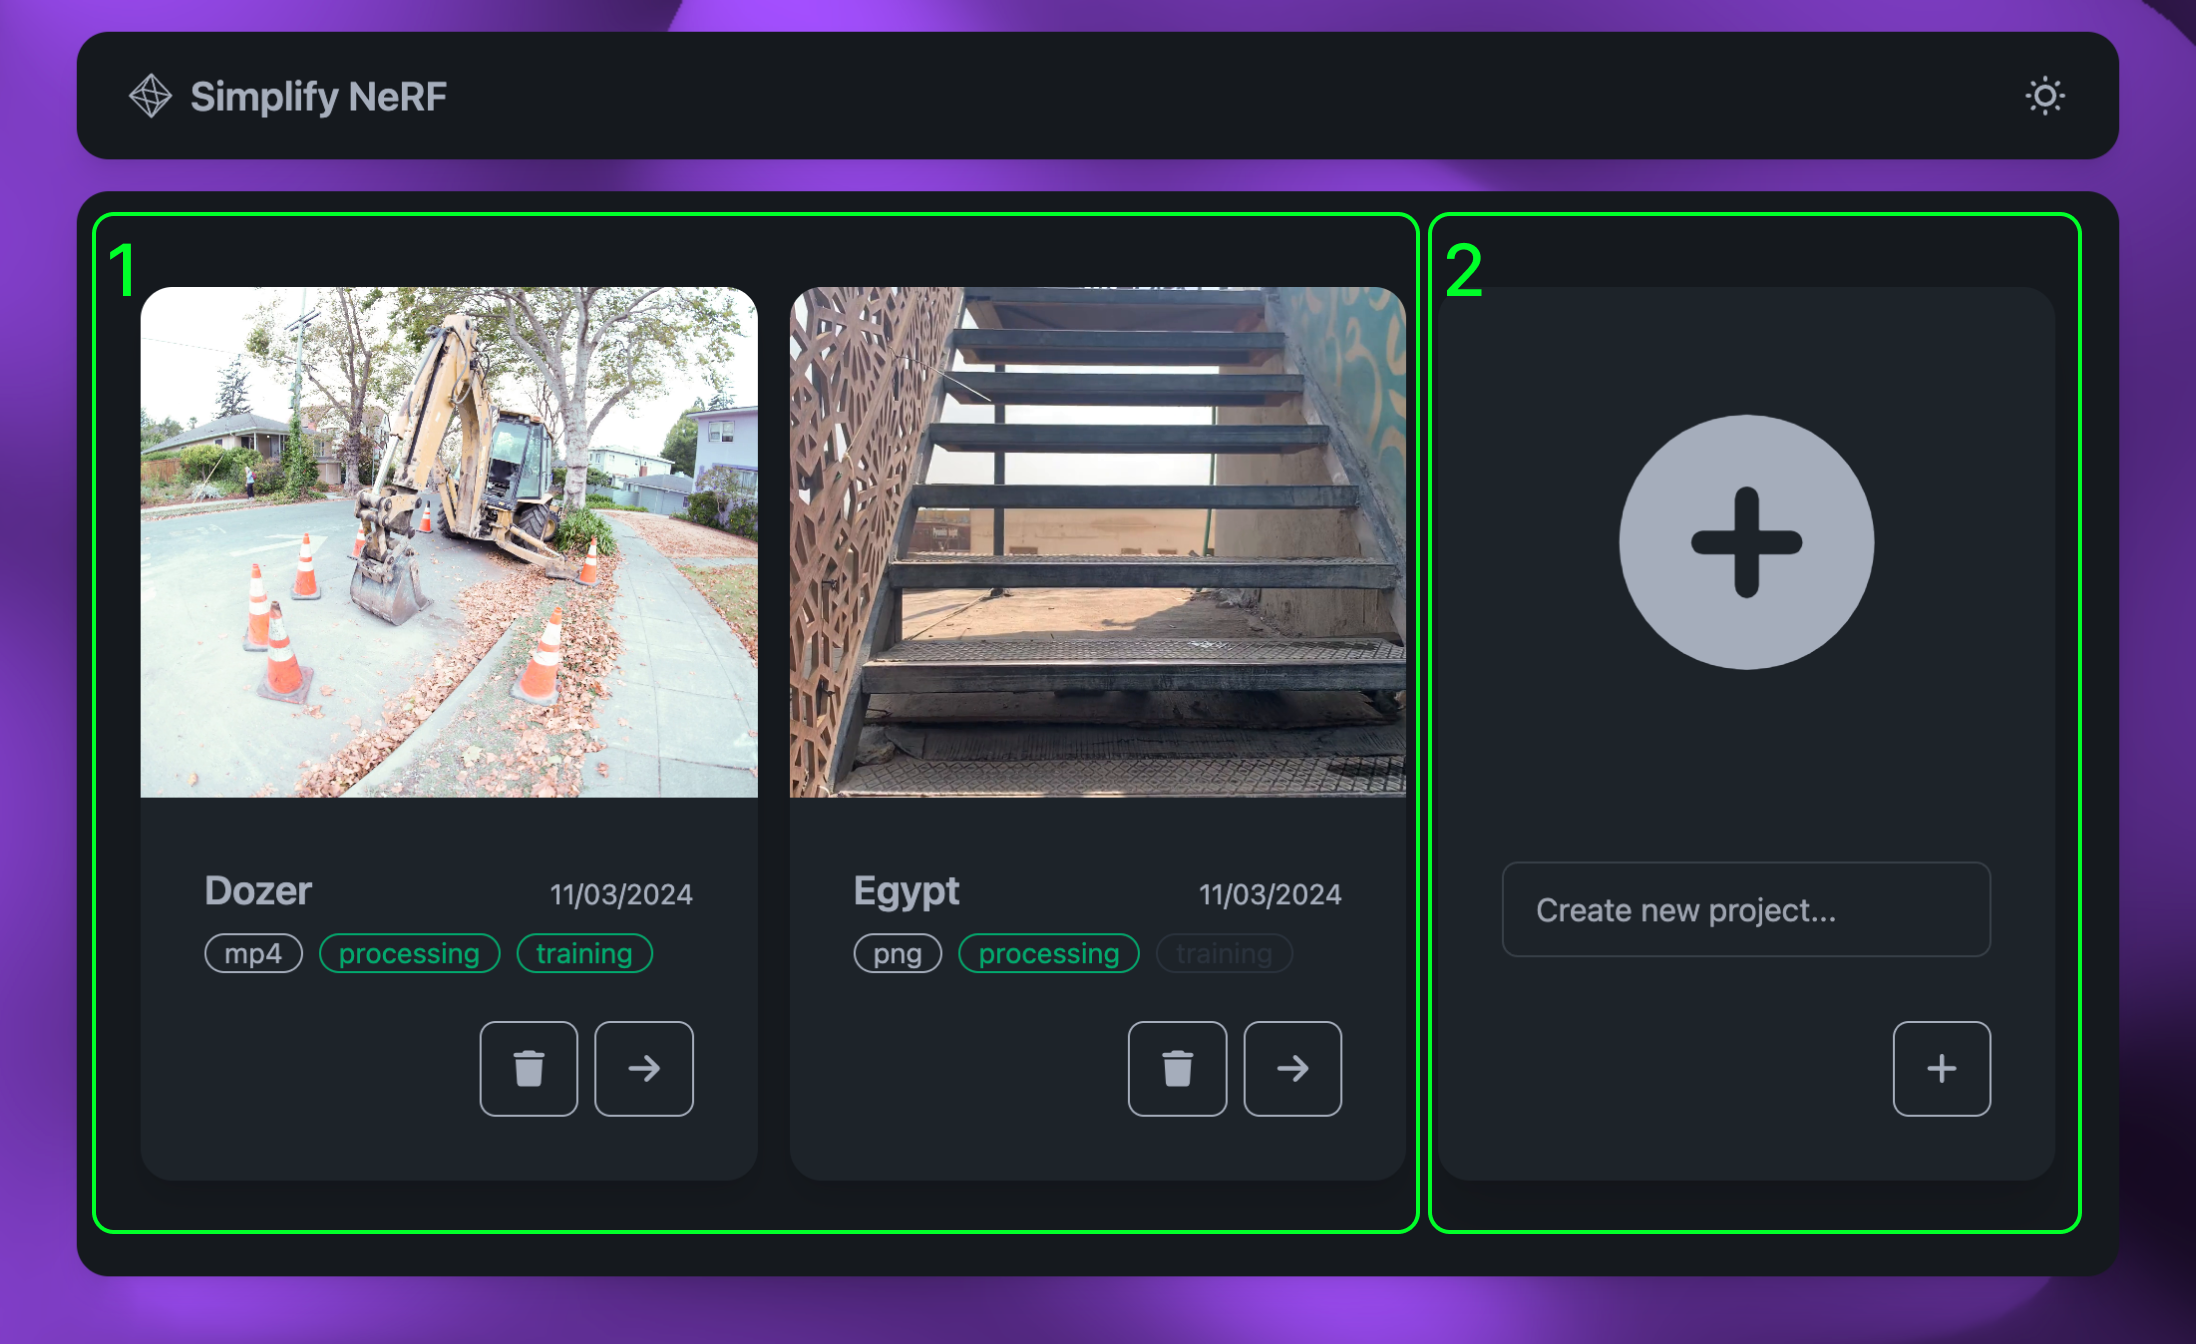
\includegraphics[width=\textwidth]{figures/view-overview.png}
  \caption{Dashboard}
  \label{fig:design:dashboard}
\end{figure}

\subsection*{Project Section}

The project section is the core of the application, through which users can create and edit NeRF models.
The section is divided into three parts: the input section, the training section, and the rendering section.
Across all sections, users user can track there progress through a progress bar at the top of the screen, that also enables easy navigation between the different sections.

\paragraph{Input Section}

The input section combines the first few interactions, as mapped out in the user flow diagram.
First users are prompted to upload there input data, which can be done by dragging and dropping files into the browser window or by clicking a button to open a file dialog.
Files can be either a set of images or a video, and there are some guardrails in place to ensure that the input data is valid.
Once the input data is uploaded, it has to be processed before it can be used for training. 
The pre-processing can be configured by the user, this includes parameters such as the lense-type, or matching method.
Parameter input fields vary based on the type of input data, and are only shown when relevant.
Once the user is satisfied with the settings, they can start the pre-processing.
Feedback on the progress of the pre-processing is given through a console that shows the output of the process running on the server.
When the pre-processing is finished, the user can move on to the training section. 

\begin{figure}[htb]
  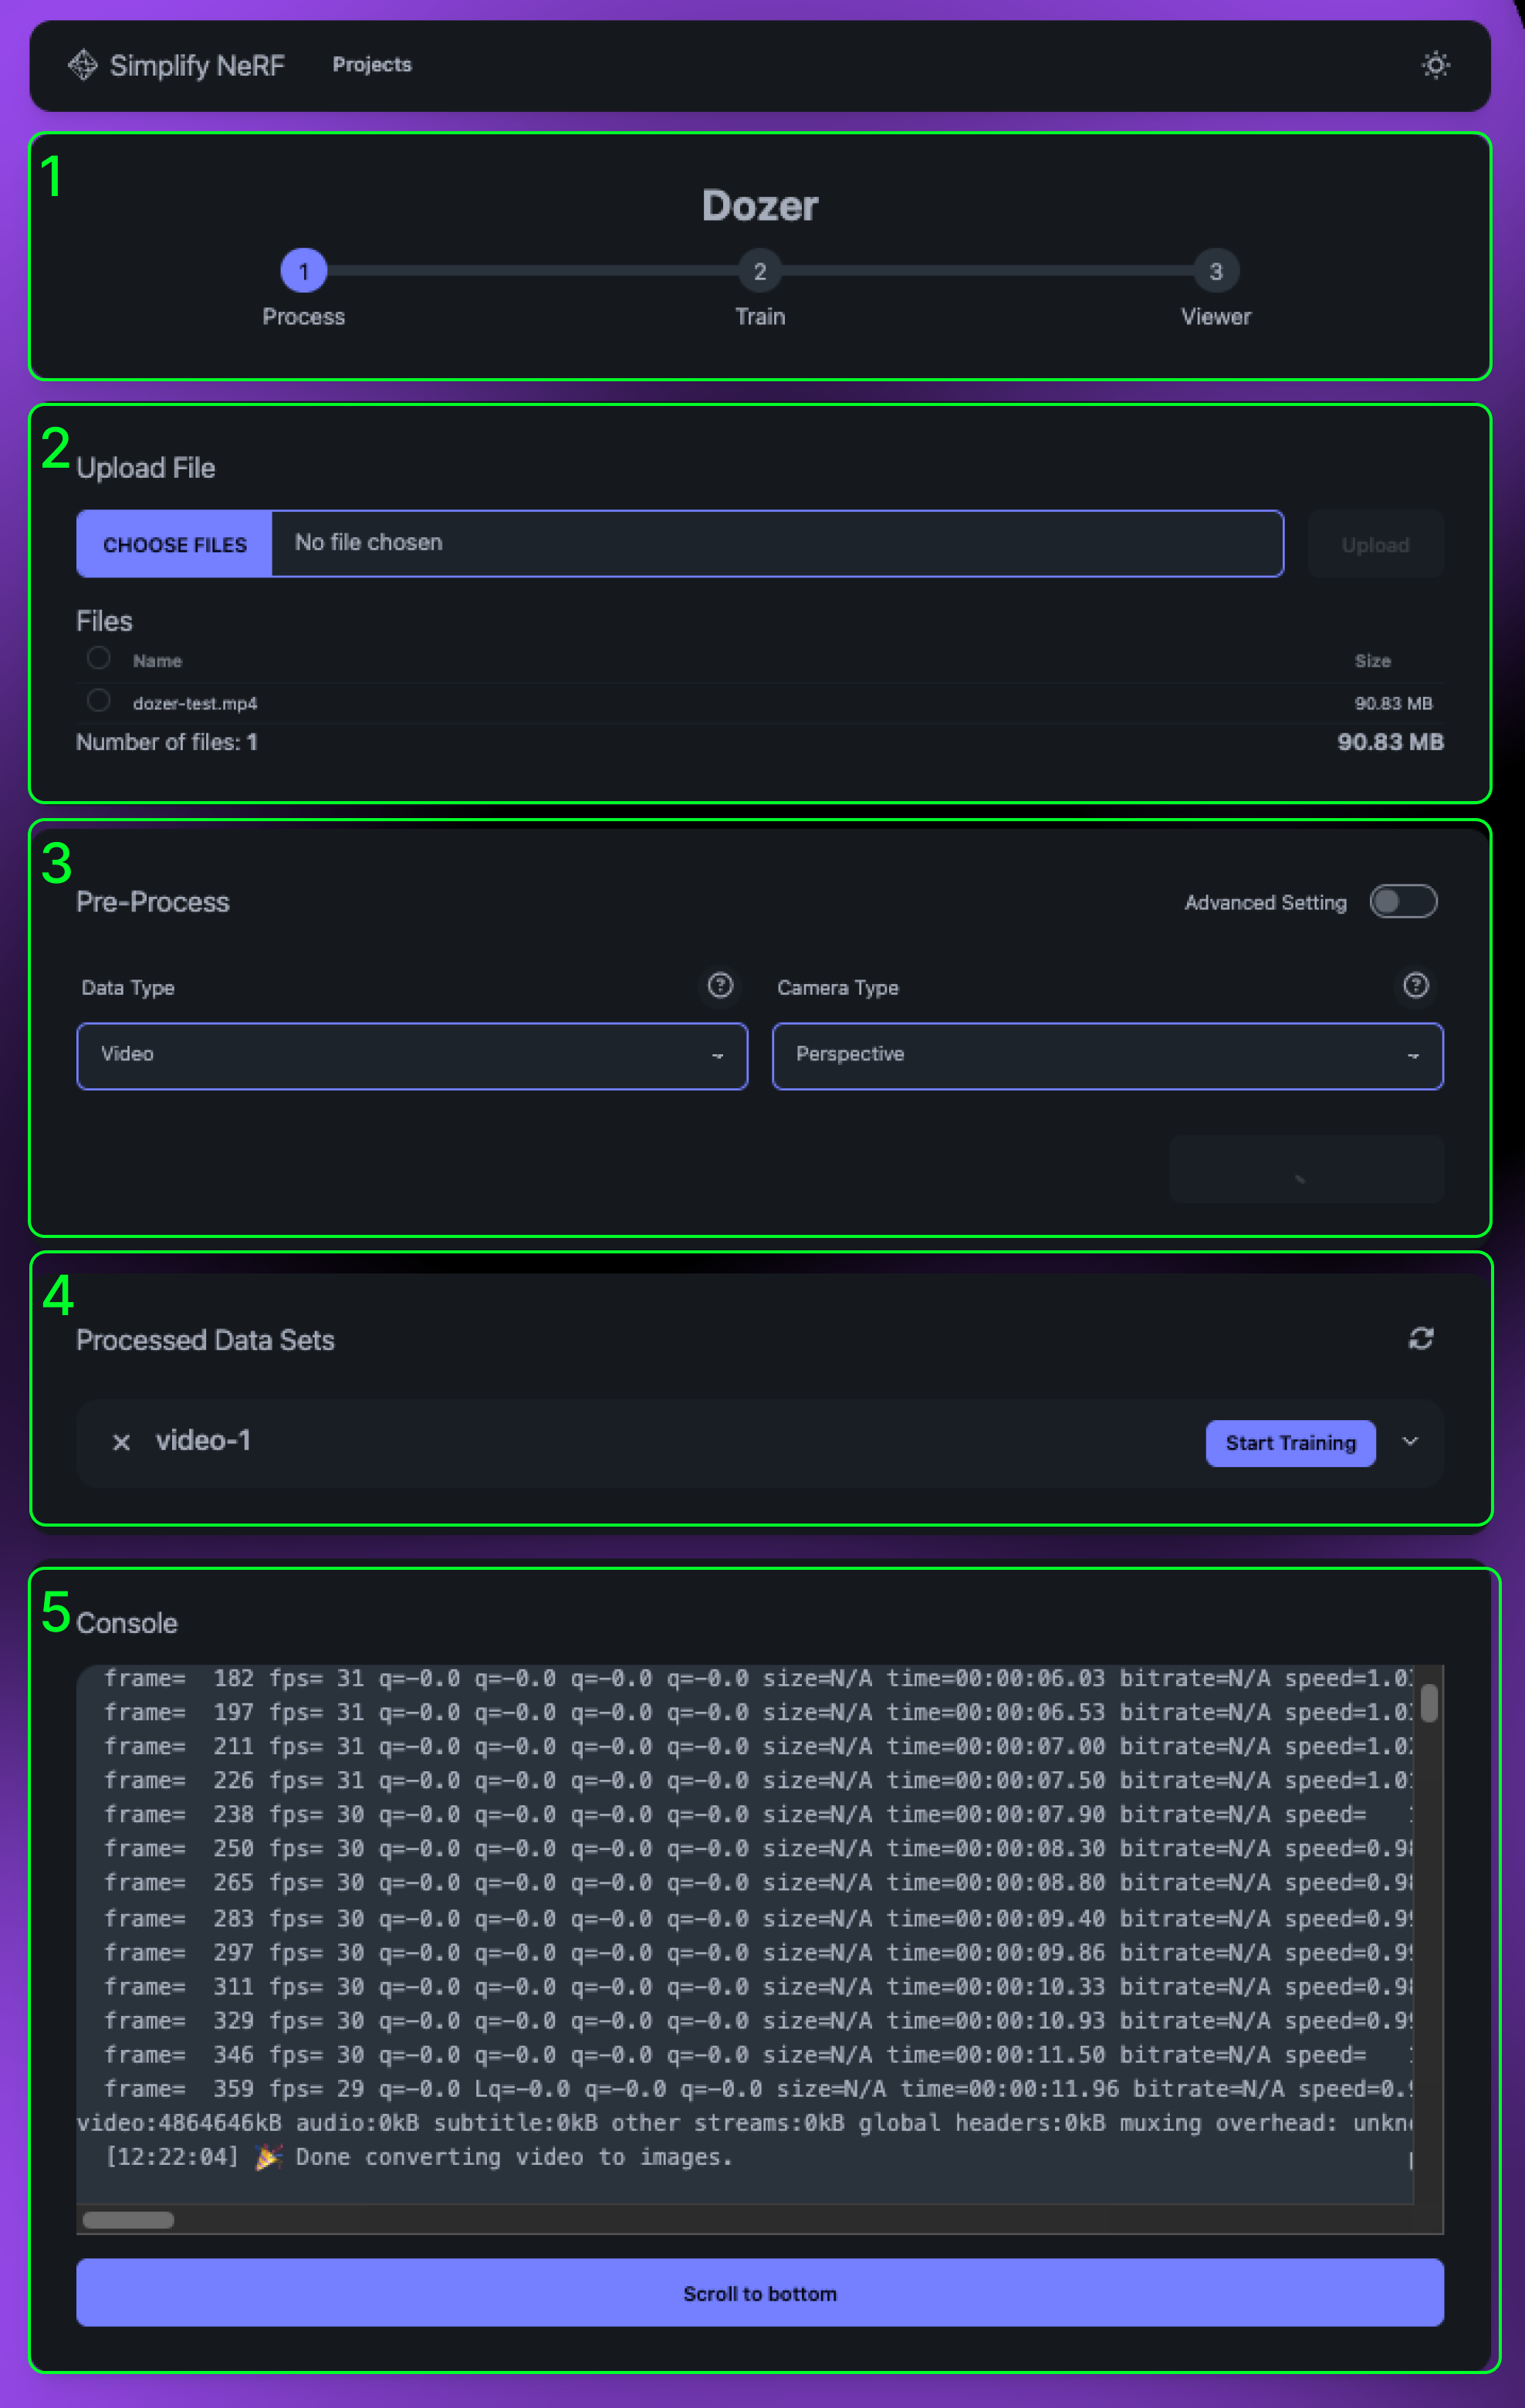
\includegraphics[width=\textwidth]{figures/view-process.png}
  \caption{Processing Input Data}
  \label{fig:design:input-section}
\end{figure}

In case the data was already pre-processed, a list ist visible that shows all available pre-processed data, and the user can select one to use for training.
Users can also inspect the configuration with which the data was pre-processed, and delete it if necessary.

\paragraph{Training Section}

The training section is structured similarly to the input section, with a form that allows users to configure the training process, and a console that shows the output of the training process running on the server.
When the user is satisfied with the configuration, they can start the training process.

\begin{figure}[htb]
  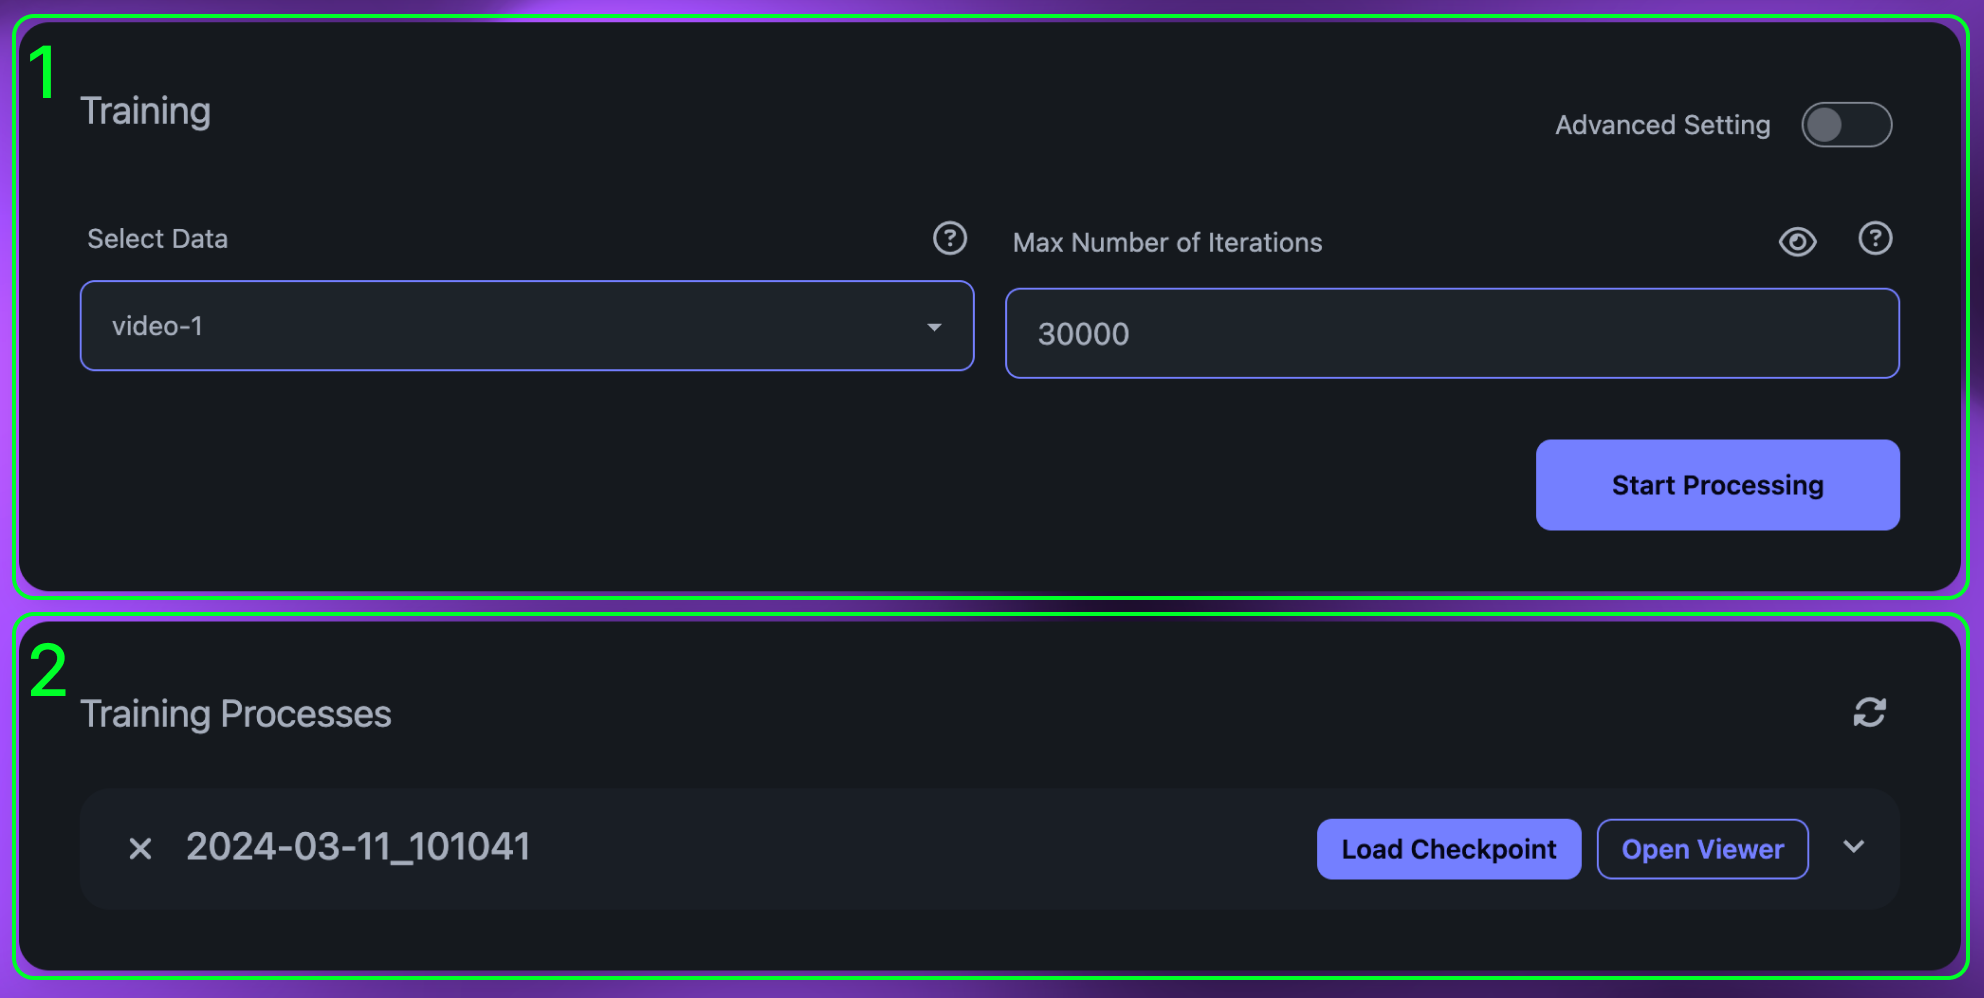
\includegraphics[width=\textwidth]{figures/view-train.png}
  \caption{Training Section}
  \label{fig:design:training-section}
\end{figure}


Previous training runs are listed, and users can inspect the configuration with which the training was run, and delete it if necessary. 
The viewer can be opened to inspect the results of the training run, or an existing checkpoint can be selected to continue training from that point.

\paragraph{Viewer Section}

The viewer section is the final step in the process, and allows users to inspect there NeRF model, while it is still training or after the training has finished.
At its core is the Nerfstudio Viewer that is integrated into the application. 
It provides users with all the functionality available in the standalone version, with a few integration that simplify the render process.
Instead of providing commands that have to be executed in the terminal, the rendering is started by clicking a button.

The renders are listed below the viewer, and once they finished processing, they can be downloaded to the users machine.

Due to the narrow layout of the page, the viewer can easily be opened in a new tab, to provide a better viewing experience.

\begin{figure}[htb]
  \includegraphics[width=\textwidth]{figures/view-viewer.png}
  \caption{Viewer Section}
  \label{fig:design:viewer-section}
\end{figure}

\subsection*{Design Language}

\paragraph{Layout}

The layout of the application is kept minimalistic, its main objective is to guide the user through the process of creating a NeRF model, and keep them informed about the progress.

All elements of interest are group together, and placed into cards to provide a clear separation between different parts of the application.
Interactions that require previous user input, appear only when necessary, and are hidden by default.
As an example, in the processing section, only the upload card is visible, until the user has uploaded some data, then the processing card appears.
This helps user to focus on the task at hand, and guide them through the process.

\paragraph{Theming}

The application support a light and a dark theme, that can be toggled by the user and uses the user's system preference as a default.
The themes are designed to be easy on the eyes, and to provide a good contrast between different elements.
Interactive elements are highlighted with a purple color, to make them stand out.

The background of the application uses a gradient animation, that is subtle and does not distract from the content, but provides a more dynamic feel to the application.
